%  \newcommand\tab[1][0,4cm]{\hspace*{#1}}
\newcommand\longtab[1][1cm]{\hspace*{#1}}

\chapter{Les technologies utilisées}
\section{Introduction}
Ces dernières années, le secteur du développement des applications mobiles a connu une majeure évolution avec l’apparition des outils de développement cross-platform. Ces outils permettent la création d’une application mobile avec une base de code unique sur les différents environnements Ios et Android. 

Au cours de ce chapitre nous allons nous présenterons d'abbord Flutter, un des frameworks utilisés pour le développement des applications multiplate-forme, ensuite nous allons parler de Firebase,  un service Google utilisé dans le côté Backend des applications. Pour finaliser nous allons définir les api Google ainsi que google maps.
\section{Flutter}
\begin{wrapfigure}[8]{r}{2cm}
    \vspace{-15pt}
    
\includegraphics[width=2cm]{images/flutterLogo.png}
    \vspace{-15pt}
\caption{{\footnotesize Logo de Flutter}}
\end{wrapfigure}
Flutter est un SDK d'application permettant de créer des applications haute performance et haute fidélité pour ios, Android, Web (version bêta) et de bureau (aperçu technique) à partir d'une base de code unique.~\cite{TechnicalOverview}
L'objectif est de permettre aux développeurs de fournir des applications hautes performances qui semblent naturelles sur différentes plateformes notamment appelés les applications multi-platformes.
\\
Flutter s’appuie sur le langage de programmation DART (à l’origine appelé Dash), créé également par Google et présenté au public en 2011.

Les applications Flutter s’exécutent dans une machine virtuelle, cette dernière offre une fonctionnalité du rechargement rapide de l’application sans avoir besoin de recompiler le projet, les applications sont donc compilées directement en code machine, sois en Javascript si elles sont destinées au web ou en instructions Intel X64 ou ARM. 
\newpage
Le framework Flutter est open source, avec une licence BSD permissive, et dispose d'un écosystème florissant de packages tiers qui complètent les fonctionnalités de base de la bibliothèque.
\begin{figure}[!h]

    \centering
    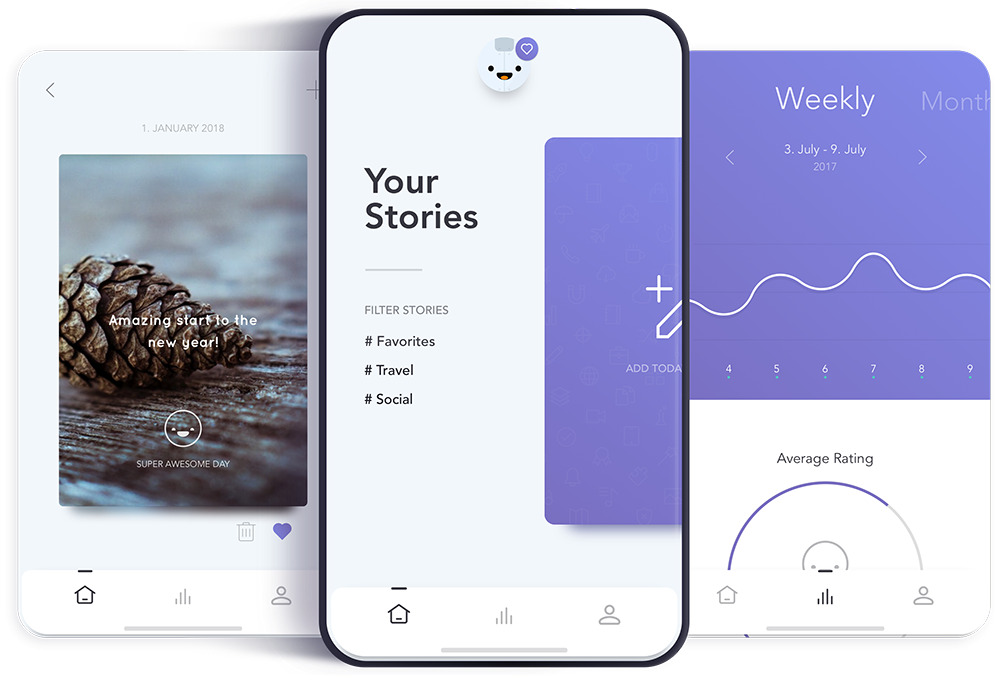
\includegraphics[width=3in]{images/Chapitre2/reflectly_app.png}
    \label{fig:firebasepricing}
    \caption{Exemple de l'application Reflectly développée avec le framework Flutter}
\end{figure}

Flutter est conçu comme un système extensible en couches. Il existe sous la forme d'une série de bibliothèques indépendantes qui dépendent chacune de la couche sous-jacente. Aucune couche n'a un accès privilégié à la couche ci-dessous, et chaque partie du niveau de structure est conçue pour être facultative et remplaçable.~\cite{FlutterArchitecturalOverview}

\begin{figure}[!h]

    \centering
    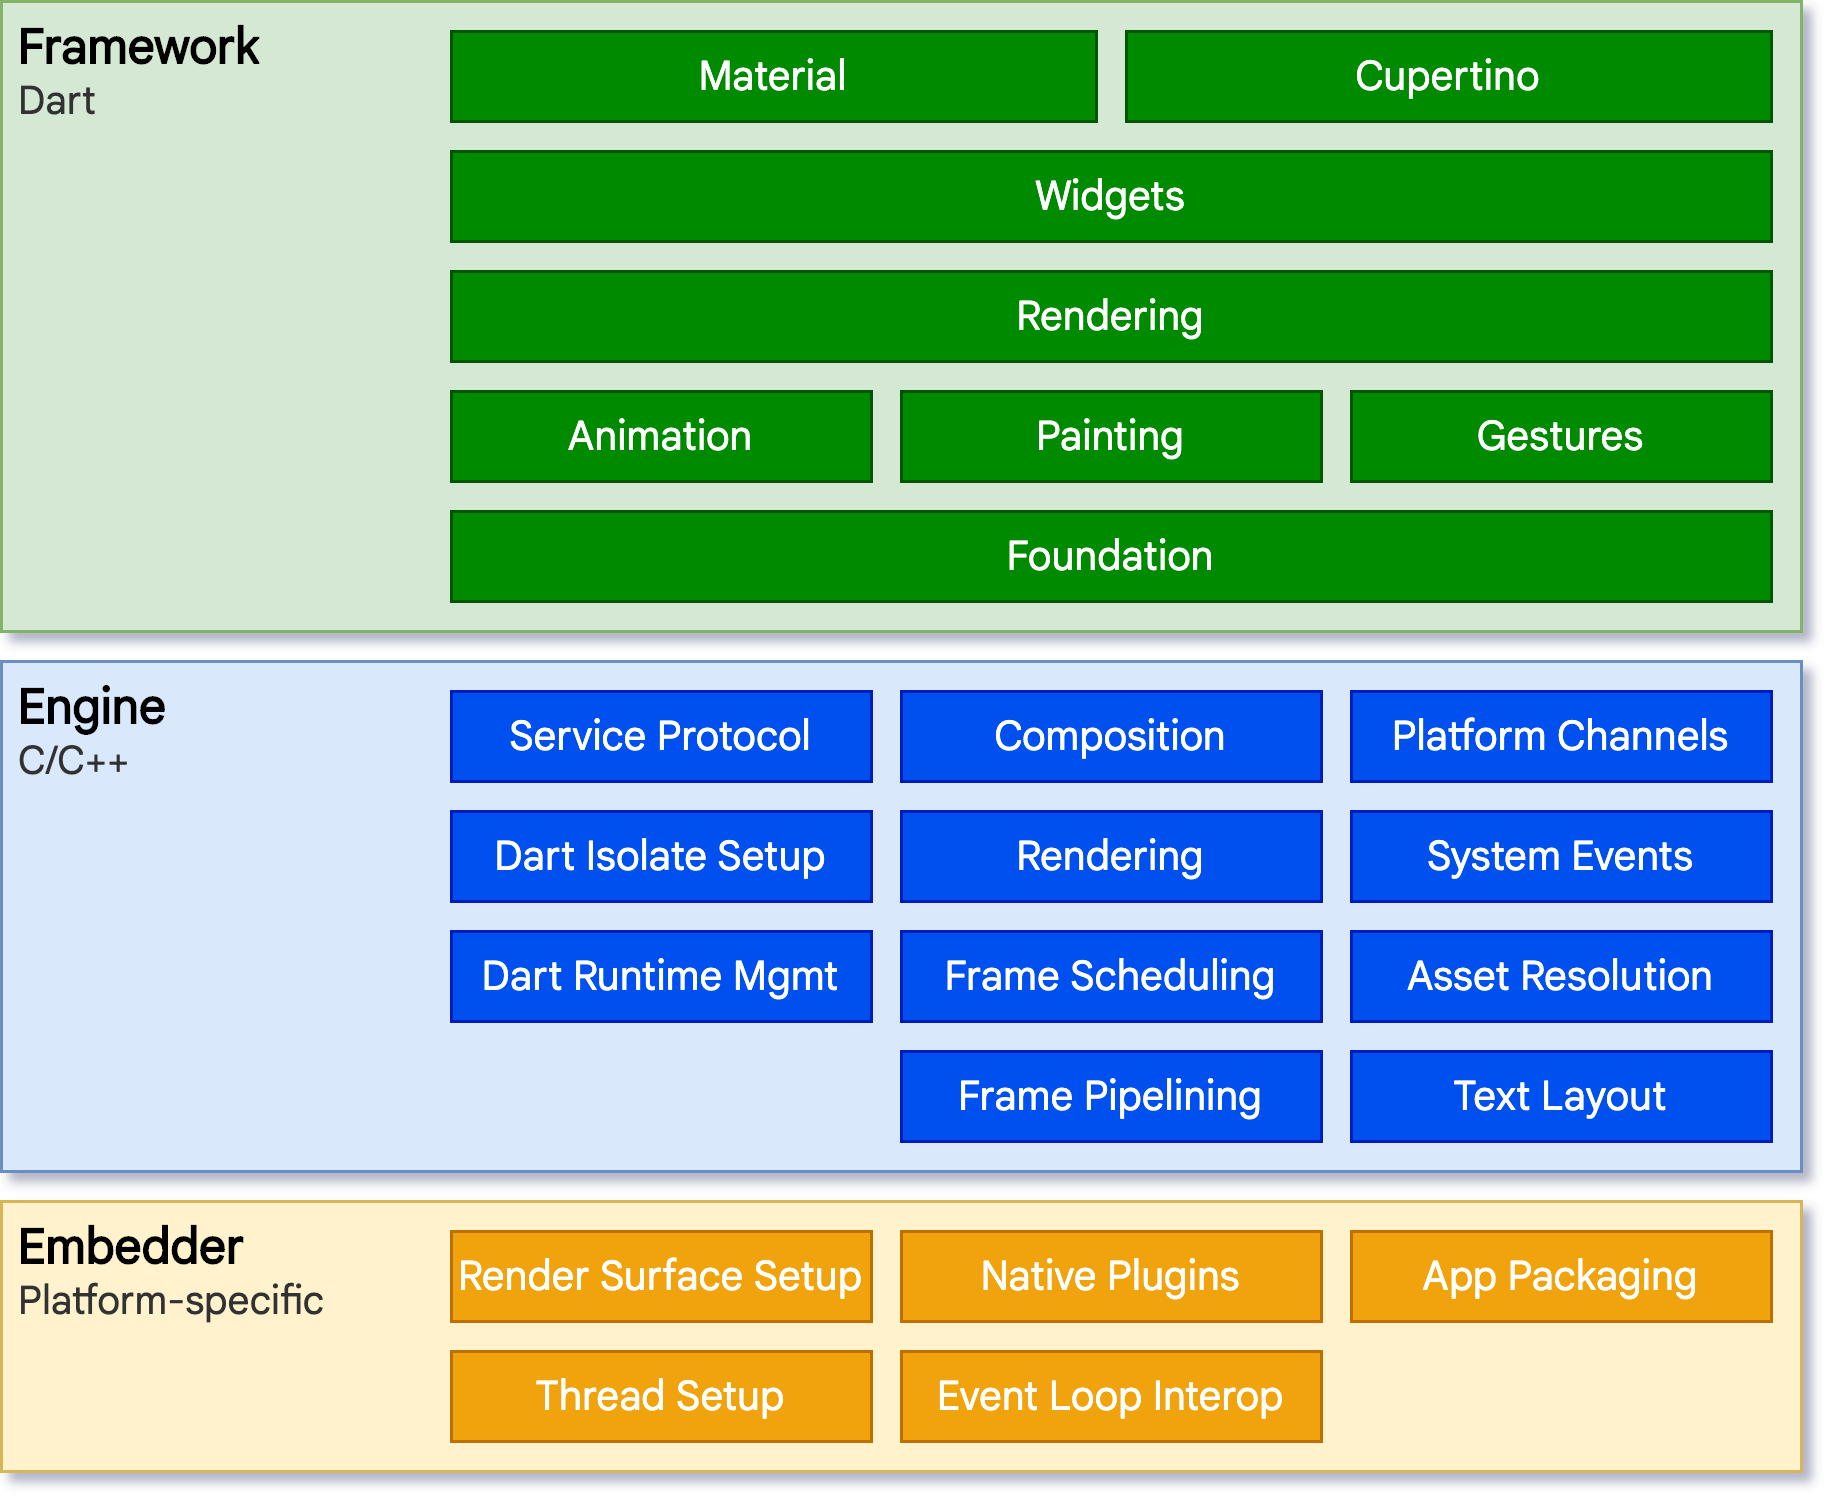
\includegraphics[width=5in]{images/Chapitre2/flutter_architectures.png}
    \label{fig:firebasepricing}
    \caption{L'architecutre du framework Flutter}
\end{figure}

\newpage


\newpage
\subsection{Principes de base}
Flutter comprend un framework de style react moderne, un moteur de rendu 2D, des widgets prêts à l’emploi et des outils de développement. Ces composants fonctionnent ensemble pour vous aider à concevoir, créer, tester et déboguer des applications.Tout est organisé autour de quelques principes fondamentaux.
\begin{enumerate}
    \item \textbf{Tout est un widget: }\\
          Les widgets sont les éléments de base de l’interface utilisateur d’une application Flutter. Chaque widget est une déclaration immuable d’une partie de l’interface utilisateur. Contrairement aux autres frameworks qui séparent les vues, les contrôleurs de vue, les présentations et d’autres propriétés, Flutter possède un modèle objet cohérent et unifié : le widget. Un widget peut
          définir :
          \begin{itemize}
              \item un élement structurel (comme un bouton ou un menu).
              \item un élement stylistique (comme une police ou un jeu de couleurs).
              \item un aspect de la mise en page (comme le rembourage).
              \item etc...
          \end{itemize} 
          
          \item \textbf{L'utilisation du language Dart}\\
       
        Le Dart est un langage de programmation structuré, open source et évolutif qui fonctionne à l'aide d'une machine virtuelle. Le projet de google à travers le Dart est de faciliter le développement web, de combler les carences du Javascript et d'offrir de meilleures performances, surtout pour les gros projets. Le Dart est destiné à fonctionner sur les navigateurs web modernes ainsi que sur les serveurs et il embarque également un convertisseur Javascript. Il y a plusieurs manières d'exécuter du code Dart; soit en utilisant un navigateur qui supporte directement ce code, soit en le compilant. En plus du navigateur Web et de la convertion javascript, le code peut être exécuté en ligne de commande, hébergé dans une machine virtuelle ce qui permet au client et au serveur d'avoir les applications écrites dans le même langage.~\cite{DartSUPINFOEcole}\bigskip
          \item \textbf{Hot Reload: }\\ 
          La fonctionnalité Hot Reload fonctionne en injectant des fichiers de code source mis à jour dans la machine virtuelle Dart (VM) en cours d'exécution. Une fois que la machine virtuelle a mis à jour les classes avec les nouvelles versions de champs et de fonctions, le framework Flutter reconstruit automatiquement l'arborescence des widgets, vous permettant de visualiser rapidement les effets de vos modifications. le build des applications est très rapide, ce qui rend quasiment invisible le temps de compilation. Un gain de temps pour les développeurs .
        \end{enumerate}          
\newpage

\subsection{Pourquoi utiliser flutter ?  }           
\textbf{-Multi-plateforme (Cross-platform)}\\
Flutter permet d'avoir une seule base de code pour tous les systèmes d'exploitation choisis. Puisque tout dans Flutter est un widget, le code est un balisage.\bigskip

\textbf{-Compatibilité avec toutes les version Android/iOS}\\
La prise en charge des applications mobiles par tous les appareils et toutes les versions du système d'exploitation est devenue un gros problème.

Ce problème a été résolu par Flutter qui a son propre moteur et des widgets pris en charge à la fois par les composants matériels pour android et Cupertino pour IOS. Les applications développées avec flutter sons prise en charge depuis la version IOS 8 et Android jelly Bean jusqu'à la dernière version.\bigskip

\textbf{-Performance et stabilité}\\
Le code de Flutter est compilé dans le code ARM du processeur. Avec son propre moteur de rendu, les applications Flutter ne sont affectées par aucune mise à jour du système d'exploitation ou personnalisation du système. Ils auront toujours la même apparence en termes d'interface même après une mise à jour du système iOS ou Android.

La compatibilité des versions est un autre aspect de l'influence de la stabilité. En tant que boîte à outils en croissance rapide, Flutter ne change pas son API et ses approches de développement. Le code écrit il y a deux ans pourrait être réutilisé dans les applications nouvellement créées.
\bigskip

% \textbf{-Productivité}\\
% Flutter offre une augmentation de la productivité qui provient
% du rechargement a chaud. Cela permet aux développeurs de voir les modifications apportée à l'état de l'application en un temps record.
 
\newpage
\section{Firebase}
\begin{wrapfigure}[8]{r}{3cm}
    \vspace{-15pt}
    
\includegraphics[width=3cm]{images/Chapitre2/firebase_logo.png}
    \vspace{-20pt}
    \caption{{\footnotesize Logo de Firebase}}
\end{wrapfigure}
Firebase est un ensemble de services d'hébergement pour n'importe quel type d'application, il propose d'héberger en NoSQL et en temps réel des bases de données,
du contenu, de l'authentification sociale (Google, Facebook, Twitter et Github),
et des notifications, ou encore des services, tel que par exemple un serveur
de communication temps réel.~\cite{Firebase2020}
\subsection{Les services de Firebase}
La platforme Firebase peut fournir trois types de services:\bigskip

\tab \textbf{1 - Construction des meilleures applications:}\bigskip

\begin{wrapfigure}[3]{l}{1cm}
 	
\includegraphics[width=1cm]{images/Chapitre2/Firebase_services/firestore.PNG}
 \end{wrapfigure}
\textbf{Cloud Firestore} Permet de stocker et synchroniser les données entre utilisateurs et appareils - à l’échelle mondiale - à l’aide d’une base de données NoSQL hébergée dans le cloud. Cloud Firestore offre donc
une synchronisation en direct et une assistance hors ligne, ainsi que
des requêtes de données efficaces. Son intégration avec d’autres produits Fi-
rebase permet de créer de véritables applications sans serveur.\medskip

\begin{wrapfigure}[3]{l}{1cm}
	
\includegraphics[width=1cm]{images/Chapitre2/Firebase_services/mlkit.PNG}
\end{wrapfigure}
\textbf{Kit ML \textsuperscript{BETA}} Ce service Apporte de puissantes fonctionnalités
d'apprentissage automatique au applications mobile. Firebase ML aide
à déployer des modèles ML personnalisés optimisés pour l'inférence sur
l'appareil, ce qui réduit la taille d'installation initiale de
l'application et permet d'effectuer plus facilement des mises à jour.
on peut également utiliser AutoML Vision Edge pour entraîner nos
propres modèles de classification d'images personnalisés ou accéder aux
API Cloud AI Vision pour une solution plus clé en main.\medskip

\begin{wrapfigure}[4]{l}{1cm}
	
\includegraphics[width=1cm]{images/Chapitre2/Firebase_services/cloud_function.PNG}
\end{wrapfigure}
\textbf{Fonctions cloud} Grace a ce service on peut devlopper les applications avec
un code backend personnalisé
sans avoir à gérer et à mettre à l'échelle nos propres serveurs.
Les fonctions peuvent être déclenchées par des événements, qui sont
émis par les produits Firebase, les services Google Cloud ou des tiers,
à l'aide de webhooks.\medskip

\begin{wrapfigure}[4]{l}{1cm}
	
\includegraphics[width=1cm]{images/Chapitre2/Firebase_services/authentication.PNG}
\end{wrapfigure}
\textbf{Authentification} Ce service permer de gérer les utilisateurs de manière simple et sécurisée.
Firebase Auth propose plusieurs méthodes pour s'authentifier,
y compris l'e-mail et le mot de passe, des fournisseurs tiers
comme Google ou Facebook, et en utilisant directement le
système de compte existant.\medskip

\begin{wrapfigure}[4]{l}{1cm}
	
\includegraphics[width=1cm]{images/Chapitre2/Firebase_services/hosting.PNG}
\end{wrapfigure}
\textbf{Hebergement} Avec ce service Firebase , l'hébergement est facile avec grace outils spécialement
conçus pour les applications Web modernes. Lorsqu'on telecharge nos
ressources Web, ces dernieres sont automatiquement transferées vers le  CDN mondial
et leur fournissons un certificat SSL gratuit afin que les utilisateurs de l'application
bénéficient d'une expérience sécurisée, fiable et à faible latence, où qu'ils se trouvent.\medskip

\begin{wrapfigure}[4]{l}{1cm}

\includegraphics[width=1cm]{images/Chapitre2/Firebase_services/cloud_storage.PNG}
\end{wrapfigure}
\textbf{Stockage en ligne} Grace a Firebase on peut Stocker et partager du contenu généré par les utilisateurs de notre application,
comme des images, de l'audio et de la vidéo avec un stockage d'objets puissant,
simple et économique conçu pour l'échelle de Google. Les SDK Firebase pour Cloud
Storage ajoutent la sécurité de Google aux importations et aux téléchargements de
fichiers pour nos applications Firebase, quelle que soit la qualité du réseau.\medskip

\begin{wrapfigure}[4]{l}{1cm}
    
\includegraphics[width=1cm]{images/Chapitre2/Firebase_services/realtime_database.PNG}
    \end{wrapfigure}
\textbf{Base de données en temps réel} Realtime Database est la base de données originale
de Firebase. C'est une solution efficace et à faible latence pour les applications
mobiles qui nécessitent des états synchronisés entre les clients en temps réel.
Le service Cloud Firestore est fortement recommendé au lieu de Realtime Database pour la plupart
des développeurs qui démarrent un nouveau projet.\bigskip

\tab \textbf{2 - Amelioaration de la qualité des applications:}\bigskip

\begin{wrapfigure}[4]{l}{1cm}
    
\includegraphics[width=1cm]{images/Chapitre2/Firebase_services/crashlytics.PNG}
    \end{wrapfigure}
\textbf{Crashlytics} Permet de réduire le temps de dépannage en transformant une avalanche
de plantages en une liste gérable de problémes. On obtien donc des informations claires et exploitable 
sur les problèmes à résoudre en premier en voyant l'impact de l'utilisateur directement dans le tableau
 de bord Crashlytics. Crashlytics est donc le principal reporter de crash de Firebase.\medskip

\begin{wrapfigure}[4]{l}{1cm}

\includegraphics[width=1cm]{images/Chapitre2/Firebase_services/performance_monitoring.PNG}
    \end{wrapfigure}
\textbf{Suivi des performances} Grace a ce service on peut diagnostiquer les problèmes de performances 
des applications survenant sur les appareils de nos utilisateurs. Donc on peut rester au courant 
de l'heure de démarrage de notre application et surveiller les requêtes HTTP sans écrire de code.\medskip

\begin{wrapfigure}[4]{l}{1cm}
    
\includegraphics[width=1cm]{images/Chapitre2/Firebase_services/test_lab.PNG}
        \end{wrapfigure}
\textbf{Laboratoire de test} Avec ce service on peut executer des tests automatiques et personnalisés pour 
notre application sur des appareils virtuels et physiques hébergés par Google.On peut alors decouvrir 
tout les bugs et les incoherences afin de pouvoir ofirir une excellent expérience au utilisateurs 
sur un large choix d'appareils .\medskip
 
\begin{wrapfigure}[4]{l}{1cm}
    
\includegraphics[width=1cm]{images/Chapitre2/Firebase_services/App_distribution.jpg}
        \end{wrapfigure}
\textbf{Distribution d'applications \textsuperscript{BETA}} Firebase App Distribution permet aux développeurs
 d'envoyer des versions préliminaires de leur application à des testeurs de confiance à partir de la console 
 ou à l'aide d'outils de ligne de commande, ainsi que de gérer les testeurs en un seul endroit.\bigskip 

\tab \textbf{3 - Developpement de l'entreprise:}\bigskip


\begin{wrapfigure}[4]{l}{1cm}
    
\includegraphics[width=1cm]{images/Chapitre2/Firebase_services/in-app_messaging.PNG}
        \end{wrapfigure}
\textbf{Messagerie integrée a l'application \textsuperscript{BETA}} Donne le pouvoir de déclencher 
des messages en fonction du comportement et des intérêts des utilisateurs. On peut aussi personnaliser
la conception des messages intégrés à l'application en fonction de notre marque. La messagerie 
intégrée prend en charge une variété de cas d'utilisation et de formats. \medskip 

\begin{wrapfigure}[4]{l}{1cm}
    
\includegraphics[width=1cm]{images/Chapitre2/Firebase_services/google_analytics.PNG}
        \end{wrapfigure}
\textbf{Google analytics} Grace aux informations en temps réel à partir de rapports on peut
Analyser les attributions et le comportement des utilisateurs et aussi exporter nos données
d'événement brutes vers Google BigQuery pour une analyse personnalisée. \medskip 

\begin{wrapfigure}[4]{l}{1cm}
    
\includegraphics[width=1cm]{images/Chapitre2/Firebase_services/a_b_testing.PNG}
        \end{wrapfigure}
\textbf{Tests A/B} L'exécution des expériences produit et marketing nous permet d'ameliorer
des tests A / B . Grace a ce service on peut personnaliser les tests en fonction de nos
objectifs et tester diverses mises à jour de notre application, comme la copie de messages
ou de nouvelles fonctionnalités. \medskip 

\begin{wrapfigure}[4]{l}{1cm}
    
\includegraphics[width=1cm]{images/Chapitre2/Firebase_services/predictions.PNG}
        \end{wrapfigure}
\textbf{Prédictions} La puissance de l'apprentissage automatique de Google est exploitée
par ce service pour obtenir des informations sur les segments d'utilisateurs susceptibles
de générer des revenus ou de dépenser (ou de terminer un autre événement de conversion).
Ces segments prédictifs intelligents peuvent etre utilisés pour cibler d'autres produits
tels que Remote Config, Cloud Messaging et In-App Messaging.\medskip 

\begin{wrapfigure}[4]{l}{1cm}
    
\includegraphics[width=1cm]{images/Chapitre2/Firebase_services/cloud_messaging.PNG}
        \end{wrapfigure}
\textbf{Messagerie Cloud} Grace a ce service on peut envoyer gratuitement des messages
et des notifications aux utilisateurs sur toutes les plates-formes (Android, iOS et 
le Web). Les messages peuvent être envoyés à des appareils uniques, à des groupes 
d'appareils ou à des sujets ou segments d'utilisateurs spécifiques. Firebase Cloud Messaging
(FCM) s'adapte même aux applications les plus volumineuses, fournissant des centaines de
milliards de messages par jour. \medskip 

\begin{wrapfigure}[4]{l}{1cm}
    
\includegraphics[width=1cm]{images/Chapitre2/Firebase_services/remote_config.PNG}
        \end{wrapfigure}
\textbf{Configuration a distance} Grace a ce service on peut personnaliser le rendu de
votre application pour chaque utilisateur, Modifier l'apparence, déployer les 
fonctionnalités progressivement, exécuter des tests A / B, fournir du contenu personnalisé
à certains utilisateurs ou effectuer d'autres mises à jour sans déployer une nouvelle
version.On peut aussi surveiller l'impact des modifications et effectuer des ajustements
en quelques minutes.\medskip 

\begin{wrapfigure}[4]{l}{1cm}
    
\includegraphics[width=1cm]{images/Chapitre2/Firebase_services/dynamic_links.PNG}
        \end{wrapfigure}
\textbf{Liens dynamiques} L'utilisation des liens dynamiques offre une expérience utilisateur
personnalisée pour iOS, Android et le Web. On les utiliser pour alimenter le Web mobile afin
de générer des conversions d'applications natives, un partage d'utilisateur à utilisateur,
des campagnes sociales et marketing, etc. Les liens dynamiques fournissent les attributions
dont on a besoin pour mieux comprendre notre croissance mobile.\medskip 
\subsection{Pourquoi utiliser Firebase ?}
Sachant que la majorité des la communité des developpeurs considére Firebase comme le Meilleur 
service BaaS (backend as a service) et l'utilise dans la majorité de leurs projets , il existe 
d'autre alternatives , parmi les alternatives on a : 

- La construction manuelle du service de gestion de l'infrastructure Backend de notre application.

\textbf{Parse :}\medskip
\begin{wrapfigure}[8]{r}{2cm}
    \vspace{-15pt}
    
\includegraphics[width=2cm]{images/Chapitre2/parse_logo.png}
    \vspace{-20pt}
    \caption{{\footnotesize Logo de Parse}}
\end{wrapfigure}
Parse est un service BaaS développé par Facebook. Parse
est un serveur Open Source, il offre donc un controle total
du code et on peut ajouter nos propre fonctions et elements. Cepandant 
l'implementation du service dans l'application reste tres difficile .

- Il existe autre alternatives comme Back4App, Backendless,
Kinvey, AWS Amplify, etc.


Cepandant, On a trouvé que Firebase est la meilleure solution a utiliser
pour notre projet pour les raisons suivantes : 

- La documentation est assez solide contrairement a parse et les autres alternatives.

- La facilité d'implementation des services d'authentification comme Google, Facebook et Github.

- La facilité de l'integration avec Flutter car Flutter et Firebase travaillent main dans la main
 pour nous aider à créer des applications mobiles en un temps record.

- La flexibilité de la tarification des services Firebase. On peut commencer gratuitement,
puis on paye au fur et à mesure celon nos besoins.~\cite{FirebasePricing}
\begin{figure}[!h]

    \centering
    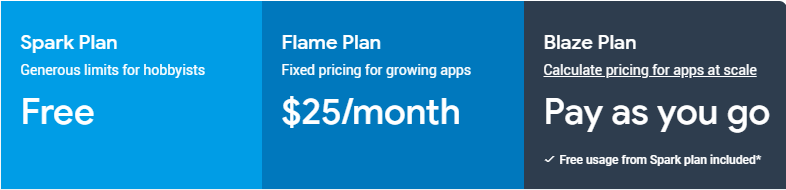
\includegraphics[width=6in]{images/Chapitre2/firebase_pricing_offers.PNG}
    \label{fig:firebasepricing}
    \caption{Exemple de la tarification d'une partie des services Firebase}
\end{figure}

\newpage

\section{Google APIs}

Les API Google sont des interfaces de programmation d'application
( API ) développées par Google qui permettent la communication avec
les services Google et leur intégration à d'autres services. Les exemples
de ceux-ci incluent la recherche, Gmail, la traduction ou Google Maps.
Les applications tierces peuvent utiliser ces API pour tirer parti ou
étendre les fonctionnalités des services existants.

Les API fournissent des fonctionnalités telles que l'analyse,
l'apprentissage automatique en tant que service (l'API de prédiction)
ou l'accès aux données utilisateur (lorsque l'autorisation de lire les
données est donnée). Un autre exemple important est une carte Google intégrée
sur un site Web, qui peut être réalisée à l'aide de l'API Static Maps,
Places API ou de l'API Google Earth .~\cite{GoogleAPIs2020}
\\
\begin{figure}[!h]

    \centering
    
\includegraphics[width=4in]{images/Chapitre2/GoogleAPIs.jpeg}
    \label{fig:googleapis}
    \caption{Logo de Google APIs}
\end{figure}
\\
Dans ce projet nous avons utilisé deux APIs : Google Maps et Google Places dont
on va en parler dans la section suivante.
\subsection{Google Maps}
Google Maps est un ervice de cartographie web,ce service disponible sur ordinateur, tablette et smartphone qui permet, à partir de l'échelle mondiale, de zoomer jusqu'à l'échelle d'une habitation.
Plusieurs types de vue sont
disponibles dans Google Maps :
une vue en plan cartographique classique,
avec les noms des rues, quartiers, villes et
une vue en images satellites ou photographies
aériennes, qui couvre aujourd'hui le monde
entier, une vue en images obliques couvrant
les grandes villes du monde et certaines
villes secondaires et une vue avec le relief.~\cite{GoogleMapsWikipedia}

Avec le SDK Maps pour Android, on peut ajouter des cartes basées
sur les données de Google Maps à notre application.
L'API gère automatiquement l'accès aux serveurs Google Maps, le
téléchargement des données, l'affichage de la carte et la réponse aux
gestes de la carte. On peut également utiliser les appels d'API pour
ajouter des marqueurs, des polygones et des superpositions à une carte de
base et pour modifier la vue de l'utilisateur d'une zone de carte
particulière. Ces objets fournissent des informations supplémentaires
sur les emplacements de la carte et permettent à l'utilisateur d'interagir
avec la carte.
\\
L'API nous permet d'ajouter ces graphiques à une carte:
\begin{itemize}
    \item Icônes ancrées à des positions spécifiques sur la carte (marqueurs).
    \item Ensembles de segments de ligne (polylignes).
    \item Segments fermés (polygones).
    \item Graphiques bitmap ancrés à des positions spécifiques sur la carte (superpositions au sol).
    \item Ensembles d'images qui sont affichés au-dessus des tuiles de la carte de base.
\end{itemize}
\begin{figure}[!h]

    \centering
    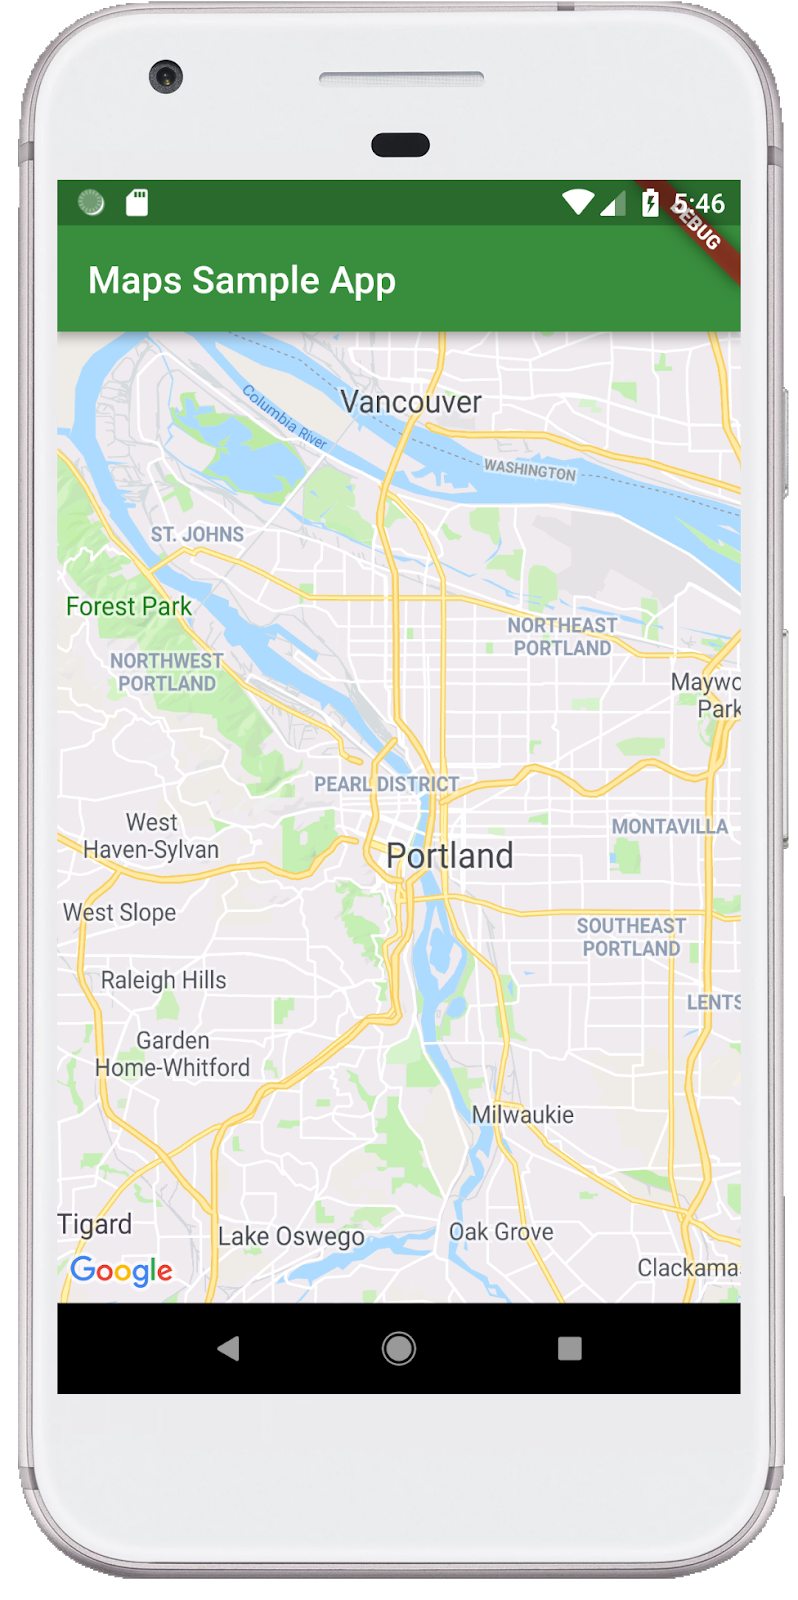
\includegraphics[width=2in]{images/Chapitre2/GoogleMapsMobile.png}
    \label{fig:GoogleMapsMobile}
    \caption{Exemple de l'integration des services Google Maps dans une application mobile}
\end{figure}
